\begin{frame}[fragile,shrink=30]
   \frametitle{Choropleth}
   Generates a choropleth map of given list of countries and indicator.`
   \begin{lstlisting}[language=Python]
    v = Visualizer('path/to/file.csv')
    fig = v.choropleth(title = '...',
                  features = 'desired_feature',
                  countries = 'all')
    fig.show() # for inline display (in browsers for example)
    \end{lstlisting}
    \begin{center}
        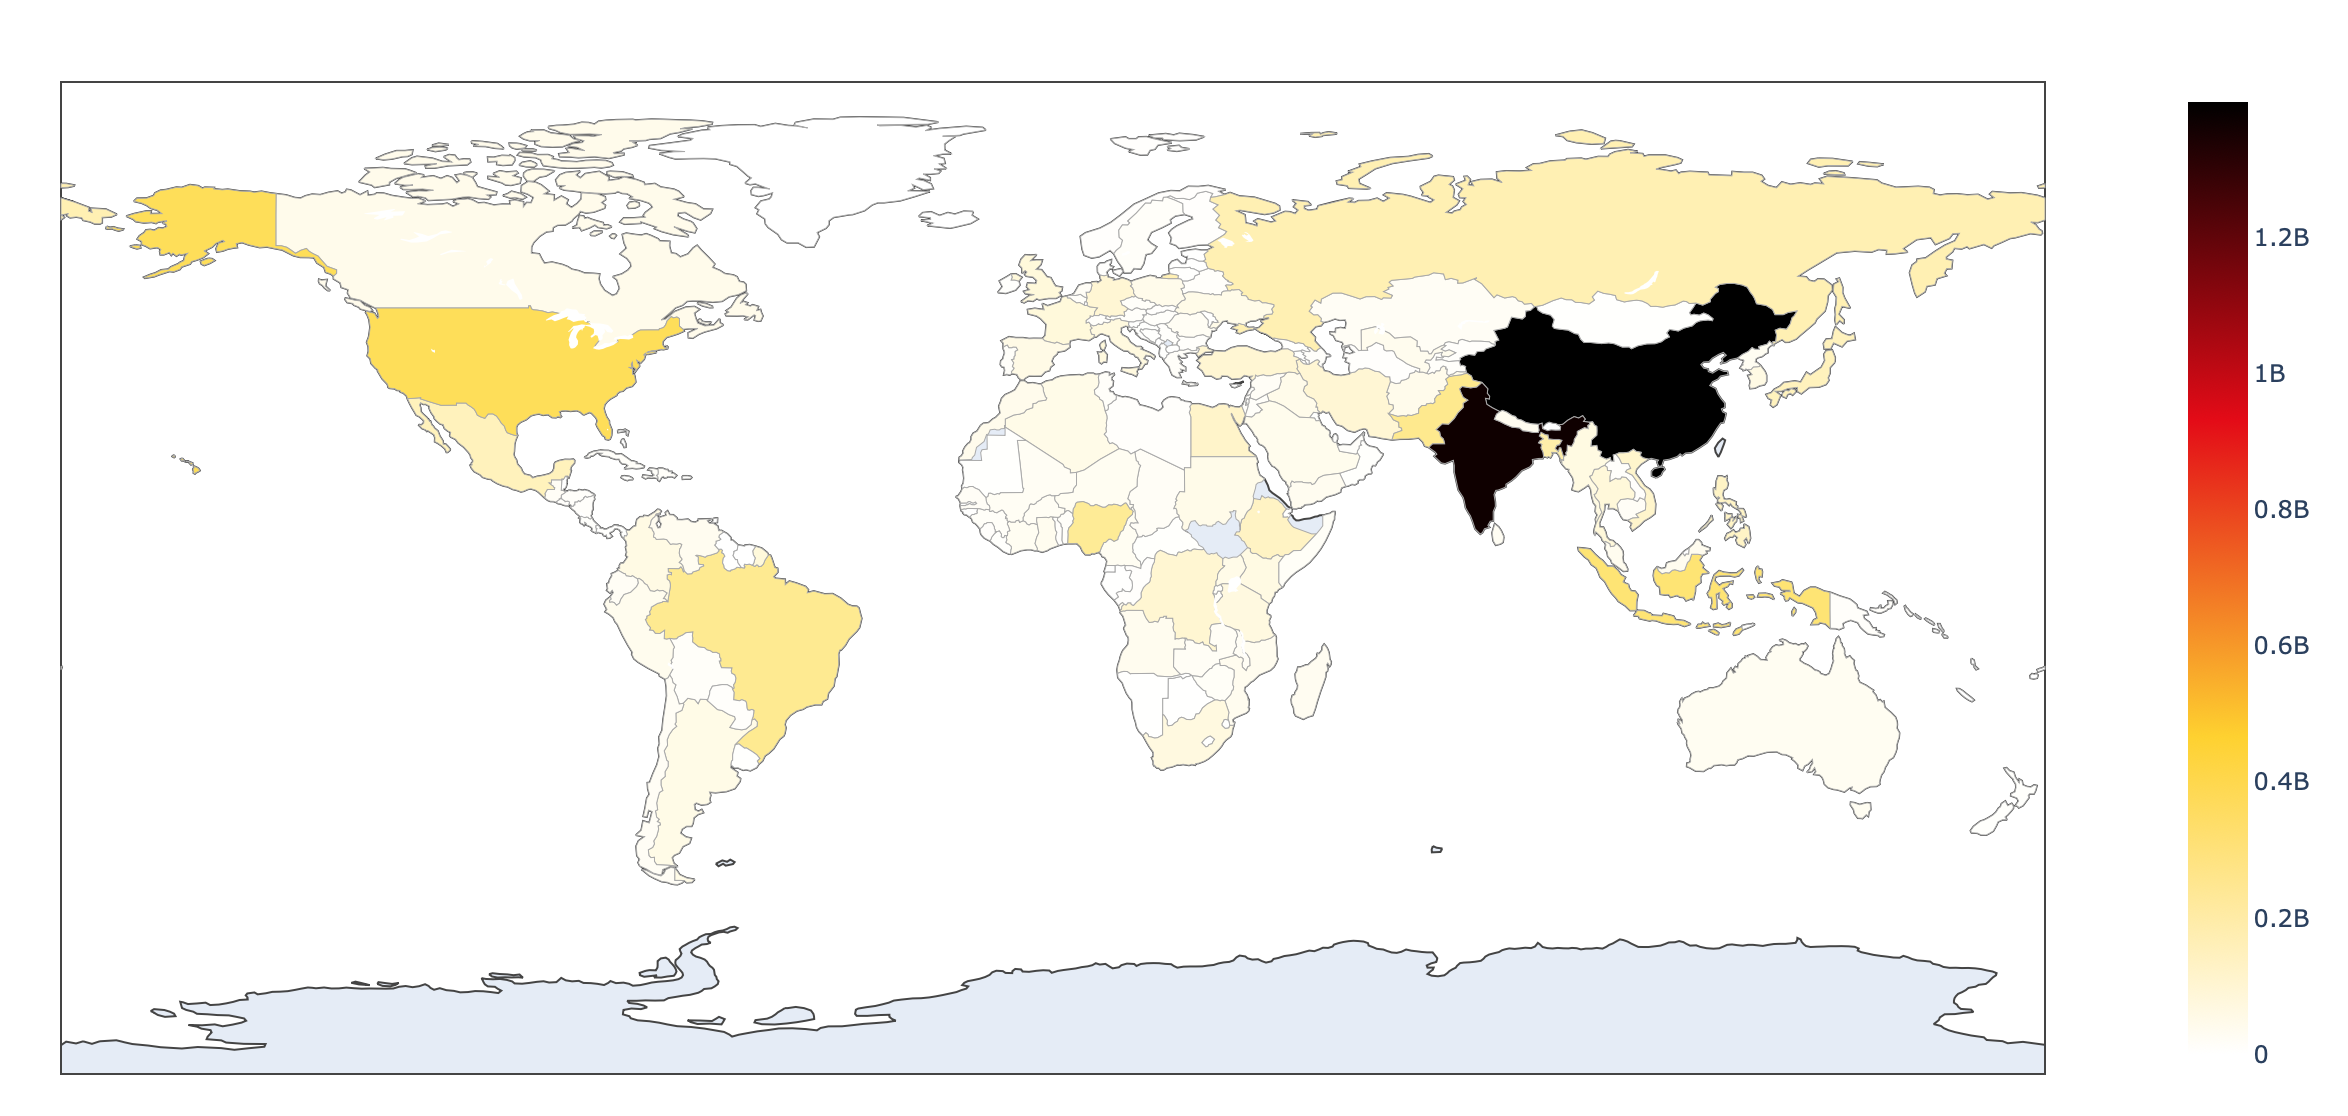
\includegraphics[scale=0.4]{beamer/inc/graphics/choropleth.png} 
    \end{center}
\end{frame}

\begin{frame}[fragile,shrink=30]
  \frametitle{Heatmap}
  Generates a heatmap correlation matrix and allows to show in a glance which countries are correlated.
  \begin{lstlisting}[language=Python]
  v = Visualizer('path/to/file.csv')
  fig = v.heatmap(countries='all', features='all',
                    method='pearson', mask=True,
                    title='This is a test heatmap', xlabel='Countries', ylabel='Countries')
  fig.show() #for inline display (in browsers for example)
  \end{lstlisting}
  \begin{center}
    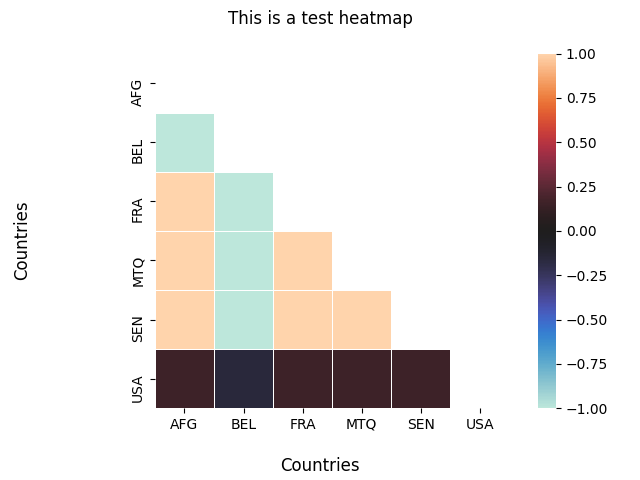
\includegraphics[scale=0.6]{beamer/inc/graphics/heatmap.png}
    \end{center}
\end{frame}

\begin{frame}[fragile,shrink=30]
  \frametitle{Time Series Plot}
  Generates a lineplot of given lists of countries and indicators.
  \begin{lstlisting}[language=Python]
    v = Visualizer('path/to/file.csv')
    fig = v.line(countries='all', features='all',
              title='This is a test of line plot', xlabel='Label of x axis', ylabel='Label of y axis', 
              legend=True)
    fig.show() # for inline display (in browsers for example)
      \end{lstlisting}
    \begin{center}
    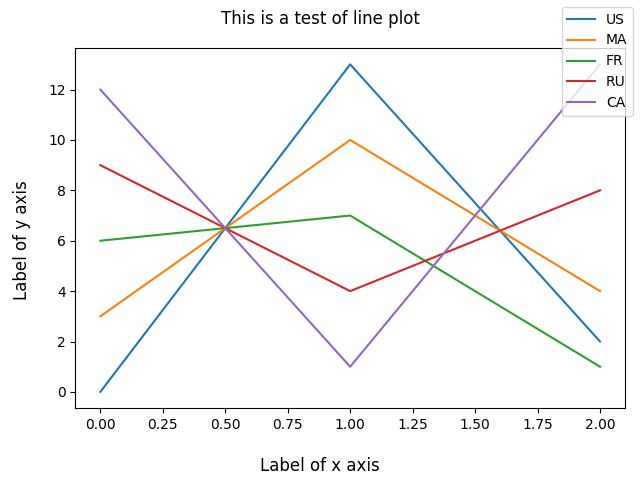
\includegraphics[scale=0.6]{beamer/inc/graphics/line.png}
    \end{center}
\end{frame}

\begin{frame}[fragile,shrink=30]
  \frametitle{Histogram}
  Generates a histogram of given lists of countries and indicators.
    \begin{lstlisting}[language=Python]
    v = Visualizer('path/to/file.csv')
    fig = v.histogram(countries=['MAR', 'CHN', 'FRA', 'RUS', 'PYF', 'SEN'], 
                    features=['f1', 'f2', 'f3'],
                    title='This is a test histogram', xlabel='Label of x axis', ylabel='Label of y axis', 
                    legend=True)
    fig.show() # for inline display (in browsers for example)
    \end{lstlisting}
    \begin{center}
    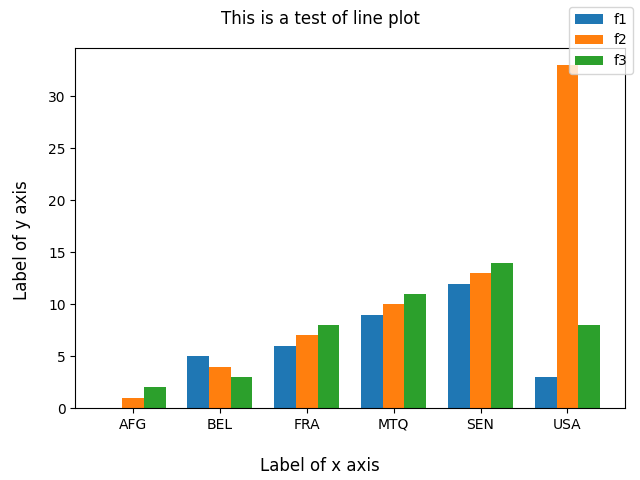
\includegraphics[scale=0.6]{beamer/inc/graphics/histogram.png}
    \end{center}
\end{frame}